\documentclass[../proyecto.tex]{memoir}

\begin{document}

\chapter{Análisis}

%\section{$\alpha$-asincronismo en la evolución de las configuraciones iniciales}

En esta sección vamos a estudiar el impacto de la $\alpha$-asíncronicidad. Las configuraciones iniciales son las escogidas en la sección \ref{seleccion}. Las ejecuciones son de 50 iteraciones con los valores de $\alpha$: 0.15, 0.3, 0.45, 0.6, 0.75, 0.9 y 0.99. Cada iteración simulada 7500 veces. Como resultado hemos obtenido los valores medios de las variables expuestas en la sección \ref{vars} junto con sus correspondientes intervalos de confianza para cada iteración.

\subsection{Hipótesis de normalidad} \label{normalidad}

Para que las estimaciones Monte Carlo tengan los intervalos de confianza de una distribución normal, es necesario comprobar que la distribución del estimador de la media sigue una distribución normal. Para ello aplicamos el de test de normalidad de Shapiro-Wilk con un nivel de significancia de 0.05, en el cual la hipótesis nula, $H_0$, es que el estimador de la media sigue una distribución normal \cite{shapiro} y la hipótesis alternativa $H_1$ [MISSING VALUE!]. Mientras que con este test no podremos afirmar que definitivamente la distribución sea normal, nos reduciremos a afirmar que no podemos afirmar que la distribución no sea normal, esto es, no rechazar la hipótesis nula. Una buena propiedad de este test, que ha motivado su elección, es que la probabilidad de rechazar la hipótesis nula cuando es cierta es aproximadamente del 5\% independientemente del tamaño de la muestra \cite{powertest}.

En la \autoref{fig:alpha} es posible observar como para cada iteración tenemos representado el intervalo de confianza $[\mu-3*\sigma, \mu+3*\sigma]$, junto con el punto central del intervalo $\mu$, la media del estimador. En las situaciones en las cuales el $p-value$ generado por el test de normalidad no supera el nivel de significación se ha pintado de color naranja, es decir, se rechaza $H_0$ y en otro caso de color azul. En caso de que la hipótesis nula sea rechazada tan solo podemos afirmar que la media del estimador converge en probabilidad como se comenta en la sección \ref{carlino}.

\begin{figure}[H]
	\centering
    \includegraphics[width=0.8\textwidth]{./images/data/lightweightspaceship/{iteracion_Area_0.30_5000_50}.png}
    \caption{Promedio de densidad para $\alpha$=0.3 de la configuración \textit{lightweight spaceship}.}
    \label{fig:alpha}
\end{figure}

Notar que para valores extremos de $\alpha$ hemos observado que se pueden encontrar situaciones en la cuales se rechaze más a menudo la hipótesis de normalidad, como las que se muestran en la \autoref{fig:tiste}. Entendemos que esta situación se puede dar por dos motivos. El primero es que si existe un número de simulaciones a partir del cual es posible dejar de negar la hipótesis de normalidad, aún no se ha alcanzado y el segundo motivo es que los valores que estemos observando sean constantes en todas las simulaciones y por tanto el estimador converge en probabilidad trivialmente como se muestra en la \autoref{fig:alpha2}.

\begin{figure}[H]
	\centering
    \includegraphics[width=0.8\textwidth]{./images/data/glider/{iteracion_Celulas_0.99_5000_50}.png}
    \caption{Promedio de nodos ocupados para $\alpha$=0.99 de la configuración \textit{glider}.}
    \label{fig:tiste}
\end{figure}


\begin{figure}[H]
	\centering
    \includegraphics[width=0.8\textwidth]{./images/data/lightweightspaceship/{iteracion_Clusteres_0.99_5000_50}.png}
    \caption{Promedio de clústeres para $\alpha$=0.99 de la configuración \textit{lightweightspaceship}.}
    \label{fig:alpha2}
\end{figure}

\subsection{\textit{Osciladores} de periodo 2} \label{osci2}

Como se observa en la \autoref{fig:blinker_evo}, cuando no existe perturbación en el intercambio de información entre nodos ocupados, el calor en cada iteración es de 4 nodos, es decir, 2 nodos se liberan y 2 nodos se ocupan iteración, ocupa un área de 3 \textit{nodos}$^2$ y está conformada por un solo clúster. En primer lugar destacamos que independientemente al valor que tome $\alpha$ el número medio de clústeres permanece constantemente 1 como se puede observar en la \autoref{fig:blinker_clusters}.

\begin{figure}[H]
	\centering
    \includegraphics[width=0.8\textwidth]{./images/data/blinker/{Clusteres_multiple_alpha}.png}
    \caption{Evolución $\alpha$-asíncrona del promedio de clústeres de la configuración \textit{blinker}.}
    \label{fig:blinker_clusters}
\end{figure}

Si observamos la \autoref{fig:blinker_calor} es posible ver que los valores medios permanecen aproximadamente constantes para cada valor de $\alpha$, además a medida que $\alpha$ se aproxima a la unidad, el promedio de calor se aproxima al que se obtiene en condiciones síncronas de evolución. También que puede observar notablemente que la variación de $\alpha$ produce que el calor medio varíe en más de 3 unidades, lo que nos hace pensar que el efecto de la $\alpha$-asincronicidad sobre esta configuración ralentiza la evolución de la misma.

Por otro lado, en la \autoref{fig:blinker_area} se observa un comportamiento más variado que el promedio de calor. Aunque se mantiene el hecho de que los valores medios de área, fijado un valor de $\alpha$, se mantienen aproximadamente constantes y también que para valores de $\alpha$ cercanos a la unidad, el promedio se aproxima al que se da bajo situación de sincronicidad, en el rango de valores de $\alpha\in[0.15,0.75]$ se observa un comportamiento diferente. En este rango, el área media crece hasta alcanzar su máximo valor cercano a 4 \textit{nodos}$^2$ cuando $\alpha$ crece hasta 0.6, sin embargo a partir de este valor de $\alpha$ los promedios comienzan a descender hasta 3.5 \textit{nodos}$^2$ en $\alpha=0.75$. Este comportamiento descrito para el área media es muy similar al que se puede observar para el número medio de vidas inmóviles (\autoref{fig:blinker_fijas}).

\begin{figure}[H]
	\centering
    \includegraphics[width=0.8\textwidth]{./images/data/blinker/{Calor_multiple_alpha}.png}
    \caption{Evolución $\alpha$-asíncrona del calor medio de la configuración \textit{blinker}.}
    \label{fig:blinker_calor}
\end{figure}

\begin{figure}[H]
	\centering
    \includegraphics[width=0.8\textwidth]{./images/data/blinker/{Area_multiple_alpha}.png}
    \caption{Evolución $\alpha$-asíncrona del área media de la configuración \textit{blinker}.}
    \label{fig:blinker_area}
\end{figure}

\begin{figure}[H]
	\centering
    \includegraphics[width=0.8\textwidth]{./images/data/blinker/{Fijas_multiple_alpha}.png}
    \caption{Evolución $\alpha$-asíncrona del número medio de vidas inmóviles de la configuración \textit{blinker}.}
    \label{fig:blinker_fijas}
\end{figure}

La densidad media en el rango de valores de $\alpha$ se puede separar en dos regiones por el valor $\alpha=0.45$, la primera donde la densidad decrece respecto de $\alpha$ y la segunda dónde ocurre lo contrario, esto es, la densidad crece hasta acercarse a valores cercanos a los que se dan con actualización síncrona. Aunque hay que notar que estas variaciones ocurren en el intervalo de valores de $[0.8, 0.95]$, luego la densidad media varía ligeramente en situación de $\alpha$-asíncronicidad.

El otro oscilador de periodo dos que hemos estudiado, la configuración \textit{toad} (\autoref{fig:toad_evo}) formada por 6 nodos ocupados que ocupan un área de 8 \textit{nodos}$^2$ en las iteraciones pares y 16 \textit{nodos}$^2$ en las impares. A diferencia de la configuración anterior tanto el área como el calor medios experimentan un comportamiento muy similar en situación de $\alpha$-asíncronicidad al que se muestra en la \autoref{fig:blinker_calor}. Comportamiento al que se suman también el número de clústeres medio que deja de ser constante y varía aproximadamente una unidad para los distintos valores de $\alpha$ (\autoref{fig:toad_clusters}). Por último la densidad media de esta configuración varía aproximadamente en el intervalo $[0.40,\ 0.65]$, observándose que el máximo valor medio se alcanza para $\alpha=0.15$ y el menor para $\alpha=0.9$, teniéndose un comportamiento decreciente respecto de $\alpha$ en los valores intermedios.


\begin{figure}[H]
	\centering
    \includegraphics[width=0.75\textwidth]{./images/data/blinker/{Fijas_multiple_alpha}.png}
    \caption{Evolución $\alpha$-asíncrona de la densidad media de la configuración \textit{blinker}.}
    \label{fig:blinker_densidad}
\end{figure}

\begin{figure}[H]
		\centering
    	\includegraphics[width=0.75\textwidth]{./images/data/toad/{Clusteres_multiple_alpha}.png}
    \caption{Evolución $\alpha$-asíncrona del número de clústeres medio de la configuración \textit{toad}.}
    \label{fig:toad_clusters}
\end{figure}

\subsection{\textit{Osciladores} de periodo 3}

En la \autoref{fig:jam_evo} podemos observar tres iteraciones de la configuración \textit{jam}, la cual curiosamente contiene una vida inmóvil. En situación de actualización síncrona esta configuración inicial está formada por 13 nodos ocupados agrupados en tres clústeres y ocupa un área de 42 \textit{nodos}$^2$. En su primera iteración se incrementa el número de nodos a 16, agrupados en un clúster y con un calor de [MISSING VALUE!] nodos, manteniendo el mismo área. La siguiente iteración incrementa su área a 49 \textit{nodos}$^2$, disminuyendo el número de nodos ocupados a 14, agrupados en dos clústeres con un calor de [MISSING VALUE!] nodos. Al avanzar una iteración más, la configuración retorna al estado de la configuración inicial. 

\begin{figure}[H]
	\centering
    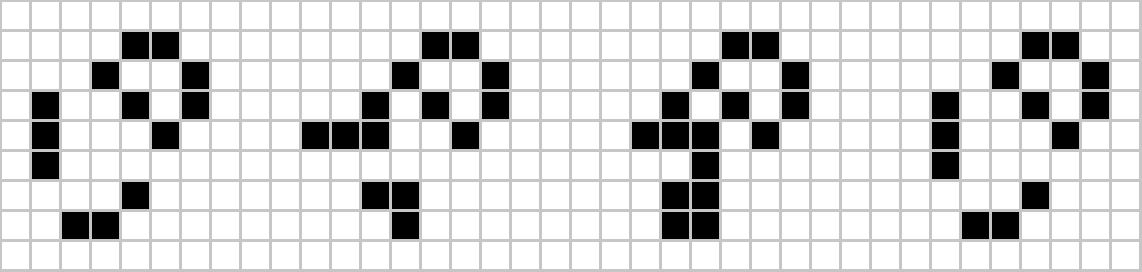
\includegraphics[width=0.9\textwidth]{./images/jam_evo.png}
    \caption{De izquierda a derecha, evolución síncrona de la configuración \textit{jam}.}
    \label{fig:jam_evo}
\end{figure}

En esta configuración se observa el mismo comportamiento para los promedios de área y calor que para la configuración \textit{toad}. Por el contrario, para el número medio de clústeres (\autoref{fig:jam_clusters}) tiene el comportamiento opuesto, esto es, el valor decrece con el crecimiento de $\alpha$, siendo su máximo y mínimo valor, cercano a 2.7 clústeres para $\alpha=0.15$ y próximo 2 clústeres para $\alpha=0.9$, respectivamente.

\begin{figure}[H]
		\centering
    	\includegraphics[width=0.8\textwidth]{./images/data/jam/{Clusteres_multiple_alpha}.png}
    \caption{Evolución $\alpha$-asíncrona del promedio de clústeres de la configuración \textit{jam}.}
    \label{fig:jam_clusters}
\end{figure}

A continuación, en la \autoref{fig:pulsar_evo} podemos observar tres iteraciones de la configuración \textit{pulsar}, la cual es notablemente la configuración de mayor tamaño que hemos estudiado. En situación de actualización síncrona esta configuración inicial está formada por 48 nodos ocupados agrupados en 12 clústeres y ocupa un área de 169 \textit{nodos}$^2$. En su primera iteración se incrementa el número de nodos a 72, agrupados en el mismo número de clústeres y con un calor de [MISSING VALUE!] nodos, incrementando el área a 225\textit{nodos}$^2$. La siguiente iteración retorna su área a 169 \textit{nodos}$^2$, manteniendo el número de nodos ocupados, agrupados en 4 clústeres con un calor de [MISSING VALUE!] nodos. Al avanzar una iteración más, la configuración retorna al estado de la configuración inicial. 

\begin{figure}[H]
	\centering
    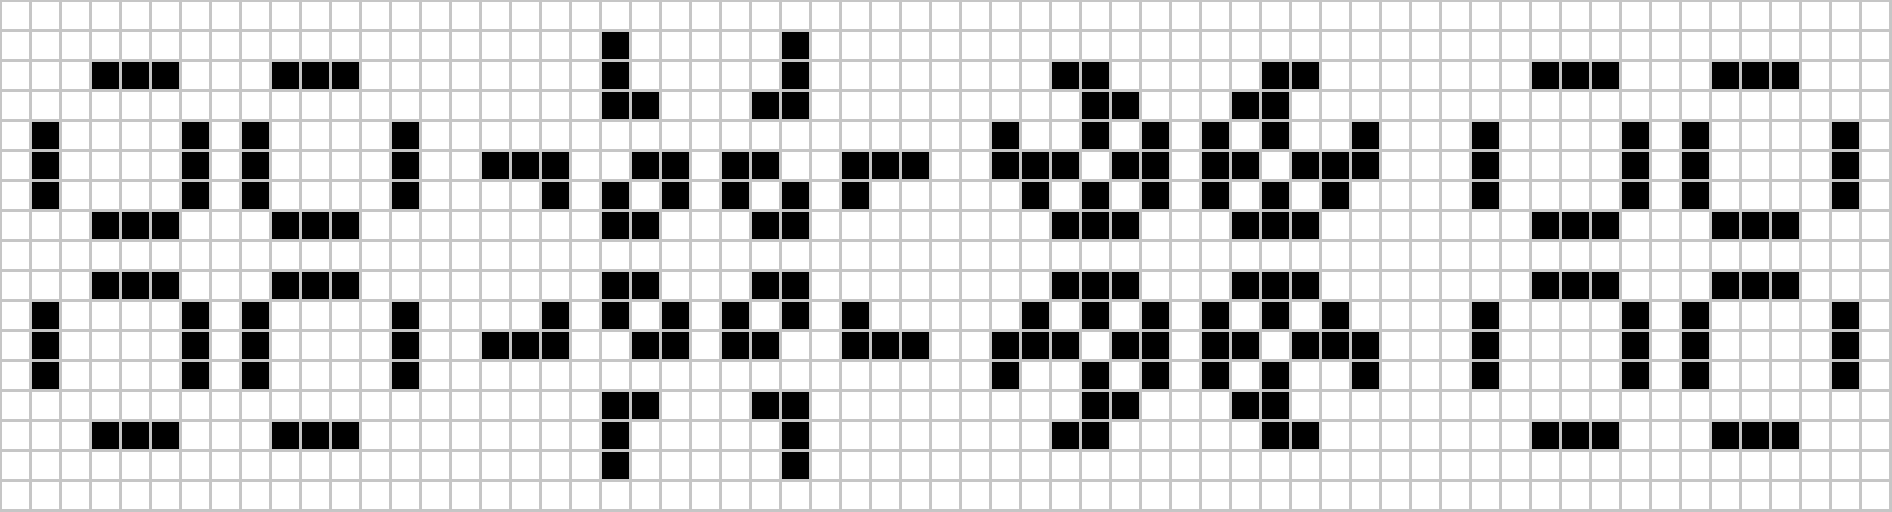
\includegraphics[width=\textwidth]{./images/pulsar_evo.png}
    \caption{De izquierda a derecha, evolución síncrona de la configuración \textit{pulsar}.}
    \label{fig:pulsar_evo}
\end{figure}

Esta configuración experimenta el mismo comportamiento en el calor medio que la configuración \textit{jam}. Por otra parte la variación de el área media (\autoref{fig:pulsar_area}) es similar, notando que la separación entre los valores medios decrece respecto de $\alpha$, alcanzando para $\alpha=0.9$ un valor medio próximo a las 225 \textit{nodos}$^2$ de la primera iteración síncrona de esta configuración. 

\begin{figure}[H]
		\centering
    	\includegraphics[width=0.8\textwidth]{./images/data/pulsar/{Area_multiple_alpha}.png}
    \caption{Evolución $\alpha$-asíncrona del promedio de área de la configuración \textit{pulsar}.}
    \label{fig:pulsar_area}
\end{figure}

El número medio de clústeres decrece de $\alpha=0.15$ a $\alpha=0.6$ una unidad, a continuación crece 1.25 clústeres de $\alpha=0.6$ a $\alpha=0.9$. Además en la (\autoref{fig:pulsar_fijas}) el número de vidas inmóviles crece casi 2 unidades respecto de $\alpha$.

\begin{figure}[H]
		\centering
    	\includegraphics[width=0.8\textwidth]{./images/data/pulsar/{Clusteres_multiple_alpha}.png}
    \caption{Evolución $\alpha$-asíncrona del promedio de clústeres de la configuración \textit{pulsar}.}
    \label{fig:pulsar_clusteres}
\end{figure}

\begin{figure}[H]
		\centering
    	\includegraphics[width=0.8\textwidth]{./images/data/pulsar/{Clusteres_multiple_alpha}.png}
    \caption{Evolución $\alpha$-asíncrona del promedio de clústeres de la configuración \textit{pulsar}.}
    \label{fig:pulsar_fijas}
\end{figure}

\subsection{\textit{Osciladores} de periodo 4}




\subsection{\textit{Naves espaciales}}
Hasta ahora solo hemos descrito el comportamiento de \textit{osciladores}. Como se expuso en la sección \ref{spaceships}, las \textit{naves espaciales} pueden ser vistas como \textit{osciladores} que se desplazan, luego es interesante explorar si los comportamientos que hemos observado en las configuraciones iniciales anteriores se reproducen en este tipo de configuraciones iniciales. 

Comenzamos la sección estudiando la configuración inicial \textit{lightweight spaceship} (\autoref{fig:lightweightspaceship}). En la \autoref{fig:lightweightspaceship_evo} se muestran 4 iteraciones de esta configuración inicial. Se trata de una configuración de velocidad $c/2$ que se desplaza paralelamente al eje horizontal con un área constante de 20 \textit{nodos}$^2$. En las iteraciones pares tiene 9 nodos ocupados agrupados en dos clústeres con un calor de [MISSING VALUE!] nodos y en las iteraciones impares tiene 12 nodos agrupados en un solo clúster con un calor de 8 nodos.

\begin{figure}[H]
	\centering
    
\includegraphics[width=\textwidth]{./images/lightweightspaceship_evo.png}
    \caption{De derecha a izquierda, evolución síncrona de la configuración \textit{lightweight spaceship}.}
    \label{fig:lightweightspaceship_evo}
\end{figure}

Uno de los característicos efectos que produce la introducción de $\alpha$-asincronismo en esta configuración inicial es que el número medio de clústeres permanece constante en todas las ejecuciones (\autoref{fig:7-1}) como en la configuración \textit{blinker}. Ésto contrasta con el hecho de que el resto de variables observadas tomen un valor diferente para cada valor de $\alpha$. Si observamos el número medio de nodos ocupados(\autoref{fig:7-2}) se observa que los valores medios se estabilizan y la separación vertical de dichos valores constantes es aproximadamente igual a 0.5 nodos ocupados entre valores consecutivos de $\alpha$. De esta manera el observamos que cuando el valor de $\alpha$ el promedio nodos ocupados se acerca a los 12 nodos ocupados en la iteraciones impares de esta configuración con la evolución síncrona.

Mientras que la densidad y el calor medios de esta configuración tienen un comportamiento similar al número medio de nodos ocupados se puede observar una variación diferente en el área media (\autoref{fig:7-3}). Cuando $\alpha$ se aproxima, tanto inferior como superiormente, a $0.5$ los valores medios de área se estabilizan entorno al valor 21.2 \textit{nodos}$^2$. Por otro lado cuando $\alpha$ se aproxima a 0 ó a 1, los valores medios se aproximan a 20.5 \textit{nodos}$^2$, un valor muy cercano a los 20 \textit{nodos}$^2$ de la configuración con evolución síncrona. Otra cuestión notable es que el valor de área media pertenece en el intervalo $(20.5, 21.5)$ cuando $\alpha$ varía, un intervalo de pequeña longitud. A diferencia de la longitud de los intervalos en los que se encuentran los promedios de nodos ocupados, densidad y calor, que es mayor.

\begin{figure}[H]
	\centering
    \includegraphics[width=0.8\textwidth]{./images/data/lightweightspaceship/{Clusteres_multiple_alpha}.png}
    \caption{Evolución $\alpha$-asíncrona del promedio de clústeres de la configuración \textit{lightweight spaceship}.}
    \label{fig:7-1}
\end{figure}

\begin{figure}[H] 
    \centering
    \includegraphics[width=0.8\textwidth]{./images/data/lightweightspaceship/{Celulas_multiple_alpha}.png}
    \caption{Evolución $\alpha$-asíncrona del promedio de nodos ocupados de la configuración \textit{lightweight spaceship}.}
    \label{fig:7-2}
\end{figure}
 
\begin{figure}[H]
	\centering
    \includegraphics[width=0.8\textwidth]{./images/data/lightweightspaceship/{Area_multiple_alpha}.png}
    \caption{Evolución $\alpha$-asíncrona del área media de la configuración \textit{lightweight spaceship}.}
    \label{fig:7-3}
\end{figure}

La configuración inicial \textit{middleweight spaceship} (\autoref{fig:middleweightspaceship}) tiene un aspecto y una evolución síncrona similar a la configuración \textit{lightweight spaceship}. En la \autoref{fig:middleweightspaceship_evo} se muestran 4 iteraciones de esta configuración inicial. Se trata de una configuración de velocidad $c/2$ que se desplaza paralelamente al eje horizontal con un área constante de 24 \textit{nodos}$^2$. En las iteraciones pares tiene 11 nodos ocupados agrupados en tres clústeres con un calor de [MISSING VALUE!] nodos y en las iteraciones impares tiene 15 nodos agrupados en un solo clúster con un calor de [MISSING VALUE!] nodos.

\begin{figure}[H]
	\centering
    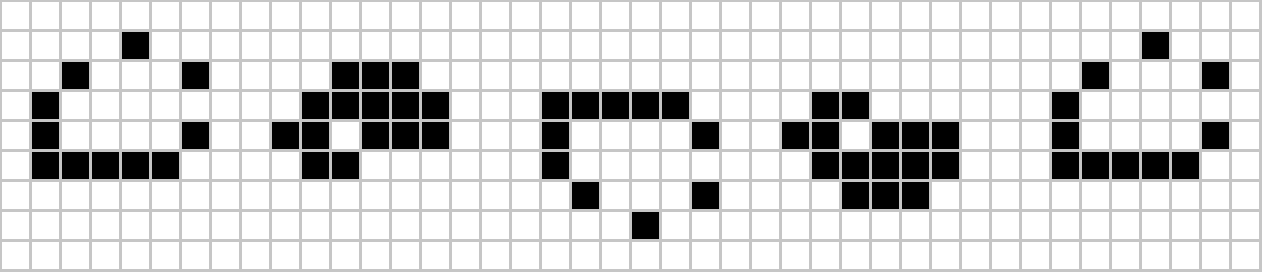
\includegraphics[width=\textwidth]{./images/middleweightspaceship_evo.png}
    \caption{De derecha a izquierda, evolución síncrona de la configuración \textit{middleweight spaceship}.}
    \label{fig:middleweightspaceship_evo}
\end{figure}

Al igual que en la configuración anterior, \textit{middleweight spaceship}, el número de clústeres permanece constante independientemente del valor de $\alpha$. Y tanto el promedio de nodos ocupados como el de densidad tienen el mismo comportamiento. Sin embargo para el valor medio de área se produce una variación del comportamiento que se puede observar en la \autoref{fig:88}. El área varía prácticamente de la misma manera para $\alpha=0.15, 0.75$ y a excepción de $\alpha=0.90$ el resto de valores de $\alpha$ muestran un comportamiento constante muy parecido entre sí a partir de la vigésima iteración. Algo que sí coincide con el comportamiento de la configuración anterior es que $\alpha=0.90$ es el promedio de área que más cercano de sitúa del valor obtenido en las iteraciones de la evolución síncrona. Otra diferencia notable es que la longitud del intervalo en el que varía el promedio crece aproximadamente una unidad.

La siguiente configuración que vamos a estudiar, \textit{heavyweight spaceship} muestra un aspecto similar a las dos anteriores tanto en forma como en su evolución síncrona. En la \autoref{fig:heavyweightspaceship_evo} se muestran 4 iteraciones de esta configuración inicial. Se trata de una configuración de velocidad $c/2$ que se desplaza paralelamente al eje horizontal con un área constante de 35 \textit{nodos}$^2$. En las iteraciones pares tiene 13 nodos ocupados agrupados en tres clústeres con un calor de [MISSING VALUE!] nodos y en las iteraciones impares tiene 18 nodos agrupados en un solo clúster con un calor de [MISSING VALUE!] nodos.

\begin{figure}[H]
	\centering
    \includegraphics[width=0.8\textwidth]{./images/data/middleweightspaceship/{Area_multiple_alpha}.png}
    \caption{Variación del área media en la configuración \textit{middleweight spaceship} para distintos valores de $\alpha$.}
    \label{fig:88}
\end{figure}

\begin{figure}[H]
	\centering
    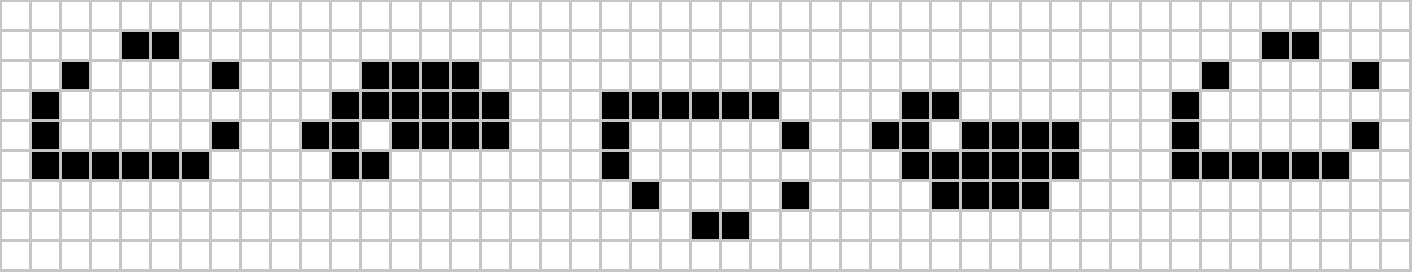
\includegraphics[width=\textwidth]{./images/heavyweightspaceship_evo.png}
    \caption{De derecha a izquierda, evolución síncrona de la configuración \textit{heavyweight spaceship}.}
    \label{fig:heavyweightspaceship_evo}
\end{figure}

A diferencia de las anteriores \textit{naves espaciales}, en la configuración \textit{heavyweight spaceship} el número de clústeres no se mantiene constante independientemente del valor que $\alpha$ tome. En la \autoref{fig:9-1} es posible observar este cambio, además todos los valores medios se mantienen aproximadamente constantes a partir de la décima iteración. A medida que $\alpha$ incrementa se visualiza que la separación vertical de los valores constantes del promedio de clústeres no es constante como en las \textit{naves espaciales} anteriores (\autoref{fig:7-2}) y dicha separación incrementa con el valor de $\alpha$.

Por otra parte, la densidad media también experimenta un comportamiento diferente en situación de $\alpha$-asincronismo en la evolución (\autoref{fig:9-2}). De nuevo a partir de la décima iteración los promedios se mantienen aproximadamente constantes pero ahora en lugar de decrecer con el crecimiento de $\alpha$, crecen de algo menos de 0.35 a algo más de 0.55 \textit{nodos}$^{-1}$.

El desarrollo en situación de $\alpha$-asincronismo que experimenta el valor medio de área es un comportamiento mucho más acentuado que los anteriores. Esto es, el intervalo en el que oscila el área media para distintos valores de $\alpha$ crece hasta una longitud de 8 \textit{nodos}$^{-1}$, siendo para $\alpha=0.9$ el menor valor de área, 31 \textit{nodos}$^2$ y para $\alpha=0.30, 0.45$ los mayores valores medios, aproximadamente 39 \textit{nodos}$^2$.

Los promedios de calor y número de nodos ocupados muestran un comportamiento idéntico al que se puede observar en la \autoref{fig:7-2}.

\begin{figure}[H]
	\centering
    \includegraphics[width=0.8\textwidth]{./images/data/heavyweightspaceship/{Clusteres_multiple_alpha}.png}
    \caption{Variación del promedio de clústeres en la configuración \textit{heavyweight spaceship} para distintos valores de $\alpha$.}
    \label{fig:9-1}
\end{figure}

\begin{figure}[H] 
    \centering
    \includegraphics[width=0.8\textwidth]{./images/data/heavyweightspaceship/{Densidad_multiple_alpha}.png}
    \caption{Variación del promedio de densidad en la configuración \textit{heavyweight spaceship} para distintos valores de $\alpha$.}
    \label{fig:9-2}
\end{figure}

Por último, la configuración inicial \textit{glider} es una nave espacial de velocidad $c/4$ formada por 5 nodos ocupados agrupados en un único clúster, tiene un calor de 4 \textit{nodos} y ocupa un área de 9 \textit{nodos}$^2$ (\autoref{fig:glider_evo}). De esta figura destacamos que el calor medio se desarrolla de forma similar al que hemos observado para la configuración \textit{blinker} al igual que lo hace el área media pero en intervalos de mayor longitud (\autoref{fig:9-3} y \autoref{fig:9-4}). Mientras que los promedios de clústeres, densidad, vidas inmóviles y nodos ocupados varían sutilmente en intervalos de muy reducida longitud.

\begin{figure}[H]
	\centering
    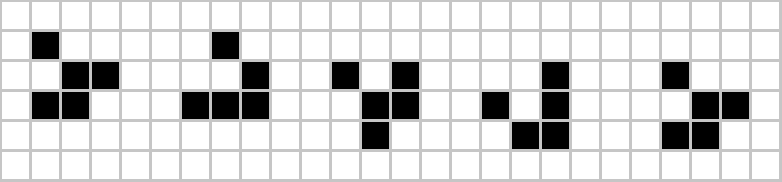
\includegraphics[width=0.8\textwidth]{./images/glider_evo.png}
    \caption{De izquierda a derecha, evolución síncrona de la configuración \textit{glider}.}
    \label{fig:lightweightspaceship_evo}
\end{figure}

\begin{figure}[H]
	\centering
    \includegraphics[width=0.8\textwidth]{./images/data/glider/{Calor_multiple_alpha}.png}
    \caption{Evolución $\alpha$-asíncrona del calor medio de la configuración \textit{glider}}
    \label{fig:9-3}
\end{figure}

\begin{figure}[H] 
    \centering
    \includegraphics[width=0.8\textwidth]{./images/data/glider/{Area_multiple_alpha}.png}
    \caption{Evolución $\alpha$-asíncrona del área media de la configuración \textit{glider}. }
    \label{fig:9-4}
\end{figure}

\end{document}